\documentclass{article}
\usepackage{graphicx} % Required for inserting images
\usepackage[top=0.9in, bottom=1in, left=1.5in, right=1.5in]{geometry}
\usepackage[utf8]{inputenc}
\usepackage[icelandic]{babel}
\usepackage[T1]{fontenc}
\usepackage[sc]{mathpazo}
\usepackage[parfill]{parskip}
\renewcommand{\baselinestretch}{1.2}
% Tables and lists
\usepackage{booktabs,tabularx}
\usepackage{multirow}
\usepackage{enumerate}
\usepackage{adjustbox}
\usepackage{multicol}
\usepackage{xcolor}
\usepackage{algpseudocode}
\usepackage{tikz}
\usepackage{nicefrac}
\usepackage{changepage}
\usetikzlibrary{arrows, positioning, calc, graphs}

% Math
\usepackage{amsmath, amsfonts, amssymb, amsthm}
% Graphics

\usepackage{graphicx}
\usepackage{hyperref}
\usepackage{tikz}
% Code environment
%\usepackage{bm}
%\usepackage{siunitx}
%\usepackage{animate}
%\usepackage{hyperref}
%\usepackage{movie15}
%\usepackage{multicol}
%\usepackage{changepage}
\title{Formal Languages and Computability 7}
\author{Ragnar Björn Ingvarsson, rbi3}
\tikzset{->, >=stealth', shorten >=1pt, node distance=2cm,thick, main node/.style={circle,draw,minimum size=3em}}

\begin{document}
\renewcommand\thepage{}
	
	\maketitle

	\newpage
	\setcounter{page}{1}
	\renewcommand\thepage{\arabic{page}}
	\setcounter{section}{2}

	\section{}
We could achieve this by first creating $1\#$ on the left side. 
Then, we could subtract the left number from the right number, check 
if the right number is all zeroes, and if not, increment the left number 
by 2 and repeat. Then, we could have an overflow checker and if it gets 
ticked, we reject.

This works on the basis that each perfect square is a sum of some 
sequential odd numbers,

\[1 = 1\]
\[4 = 1 + 3\]
\[9 = 1 + 3 + 5\]
\[16 = 1 + 3 + 5 + 7\]

and so on.
	\section{}
	\begin{itemize}
		\item[a)] We can show that $A$ is regular by creating a NFA that 
			describes the language.
			\vspace{2em}
			\begin{center}
			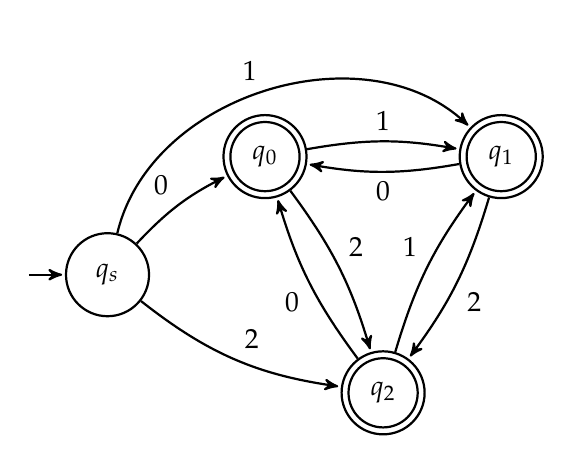
\begin{tikzpicture}[thick,auto]
				\node[main node] at (-2,-1.5) (qs) {$q_s$};
				\node[main node] (q0) {$q_0$};
				\node[main node] at (3,0) (q1) {$q_1$};
				\node[main node] at (1.5,-3) (q2) {$q_2$};
				\node[main node,minimum size=2.5em] (q0fin) {};
				\node[main node,minimum size=2.5em] at (3,0) (q1fin) {};
				\node[main node,minimum size=2.5em] at (1.5,-3) (q2fin) {};

				\path (-3,-1.5) edge node {} (qs);
				\path (qs) edge[bend left=10] node {$0$} (q0);
				\path (qs) edge[bend left=60] node {$1$} (q1);
				\path (qs) edge[bend right=15] node {$2$} (q2);
				\path (q0) edge[bend left=10] node {$1$} (q1);
				\path (q0) edge[bend left=10] node {$2$} (q2);
				\path (q1) edge[bend left=10] node {$2$} (q2);
				\path (q1) edge[bend left=10] node {$0$} (q0);
				\path (q2) edge[bend left=10] node {$0$} (q0);
				\path (q2) edge[bend left=10] node {$1$} (q1);
			\end{tikzpicture}
			\end{center}

			Here we have a NFA that only accepts a string where from 
			a recent 0,1,2 we can only accept numbers that are not the 
			most recent number.
		\item[b)] This can be solved by first reading the tape and 
			determining if the string is in $A$ and reject it if so, as 
			per the question on ed, \url{https://edstem.org/eu/courses/1535/discussion/134577}. Then, we could create three spaces on the left side of 
			the input string, for counting the occurrences of each symbol 
			with a binary number. 
			Then we run through the string, replacing each read symbol with 
			say, an $X$, and incrementing the corresponding counter. At the end, we have our three binary numbers 
			representing the number of symbols of each kind and we can 
			compare the three to ensure that no symbol occurrs more than 
			the other two combined plus $1$.
	\end{itemize}


\end{document}
